\documentclass[11pt]{article}
\usepackage[left=3cm,right=3cm,top=3cm,bottom=3cm]{geometry}
\usepackage{url}
\usepackage{amssymb}
\usepackage{mathrsfs, bm}
\usepackage{enumitem}
\usepackage{array}
\usepackage{graphicx}
\graphicspath{ {./images/} }

\usepackage{titlesec}
\newcommand{\sectionbreak}{\clearpage}

\begin{document}
\title{COMP0123 Complex Networks and Webs Coursework 1 Report}
\author{Roman Ryan Karim}
\date{October 24, 2023}
\maketitle

\section*{Task 1 - (15 marks)}

\fbox{%
  \parbox{1\textwidth}{%
  \begin{itemize}
	\item Calculate the average node degree and the maximum node degree of the 3 networks.
	\item Plot their degree distribution $P(k)$ on linear-linear scale and log-log scale, respectively.
	\item Estimate the power-law exponent of the degree distribution $P(k)$ of the author network only.
	\begin{itemize}
		\item You can fit a curve by using the function polyfit from the numpy library.
		\item Ideally, you can do the fitting on CCDF (the complementary cumulative distribution function) on log-log scale.
	\end{itemize}
	\item Briefly discuss your results, e.g. difference of the networks.
\end{itemize}}%
}

\paragraph{}The average node degree is given by $\bar{k} = \frac{1}{N}\sum^{N}_{i = 1} = \frac{2E}{N}$. Given that all 3 of our networks (author network, random network \& BA network) have 2,068 unique nodes and 5,163 unique links;  $\bar{k} = \frac{2(5163)}{2068} = 4.99$ (2 d.p.).

\begin{center}
\begin{tabular}{ | m{12em} | m{12em} | m{12em} | } 
  \hline
  \textbf{Networks} & \textbf{Average Node Degree} & \textbf{Maximum Node Degree}\\
  \hline 
  Author Network & 4.99 & 51 \\ 
  \hline
  Random Network & 4.99 & 13 \\ 
  \hline
  BA Network & 4.99 & 48 \\
  \hline
\end{tabular}
\end{center}

\begin{figure}[h]
    \centering
    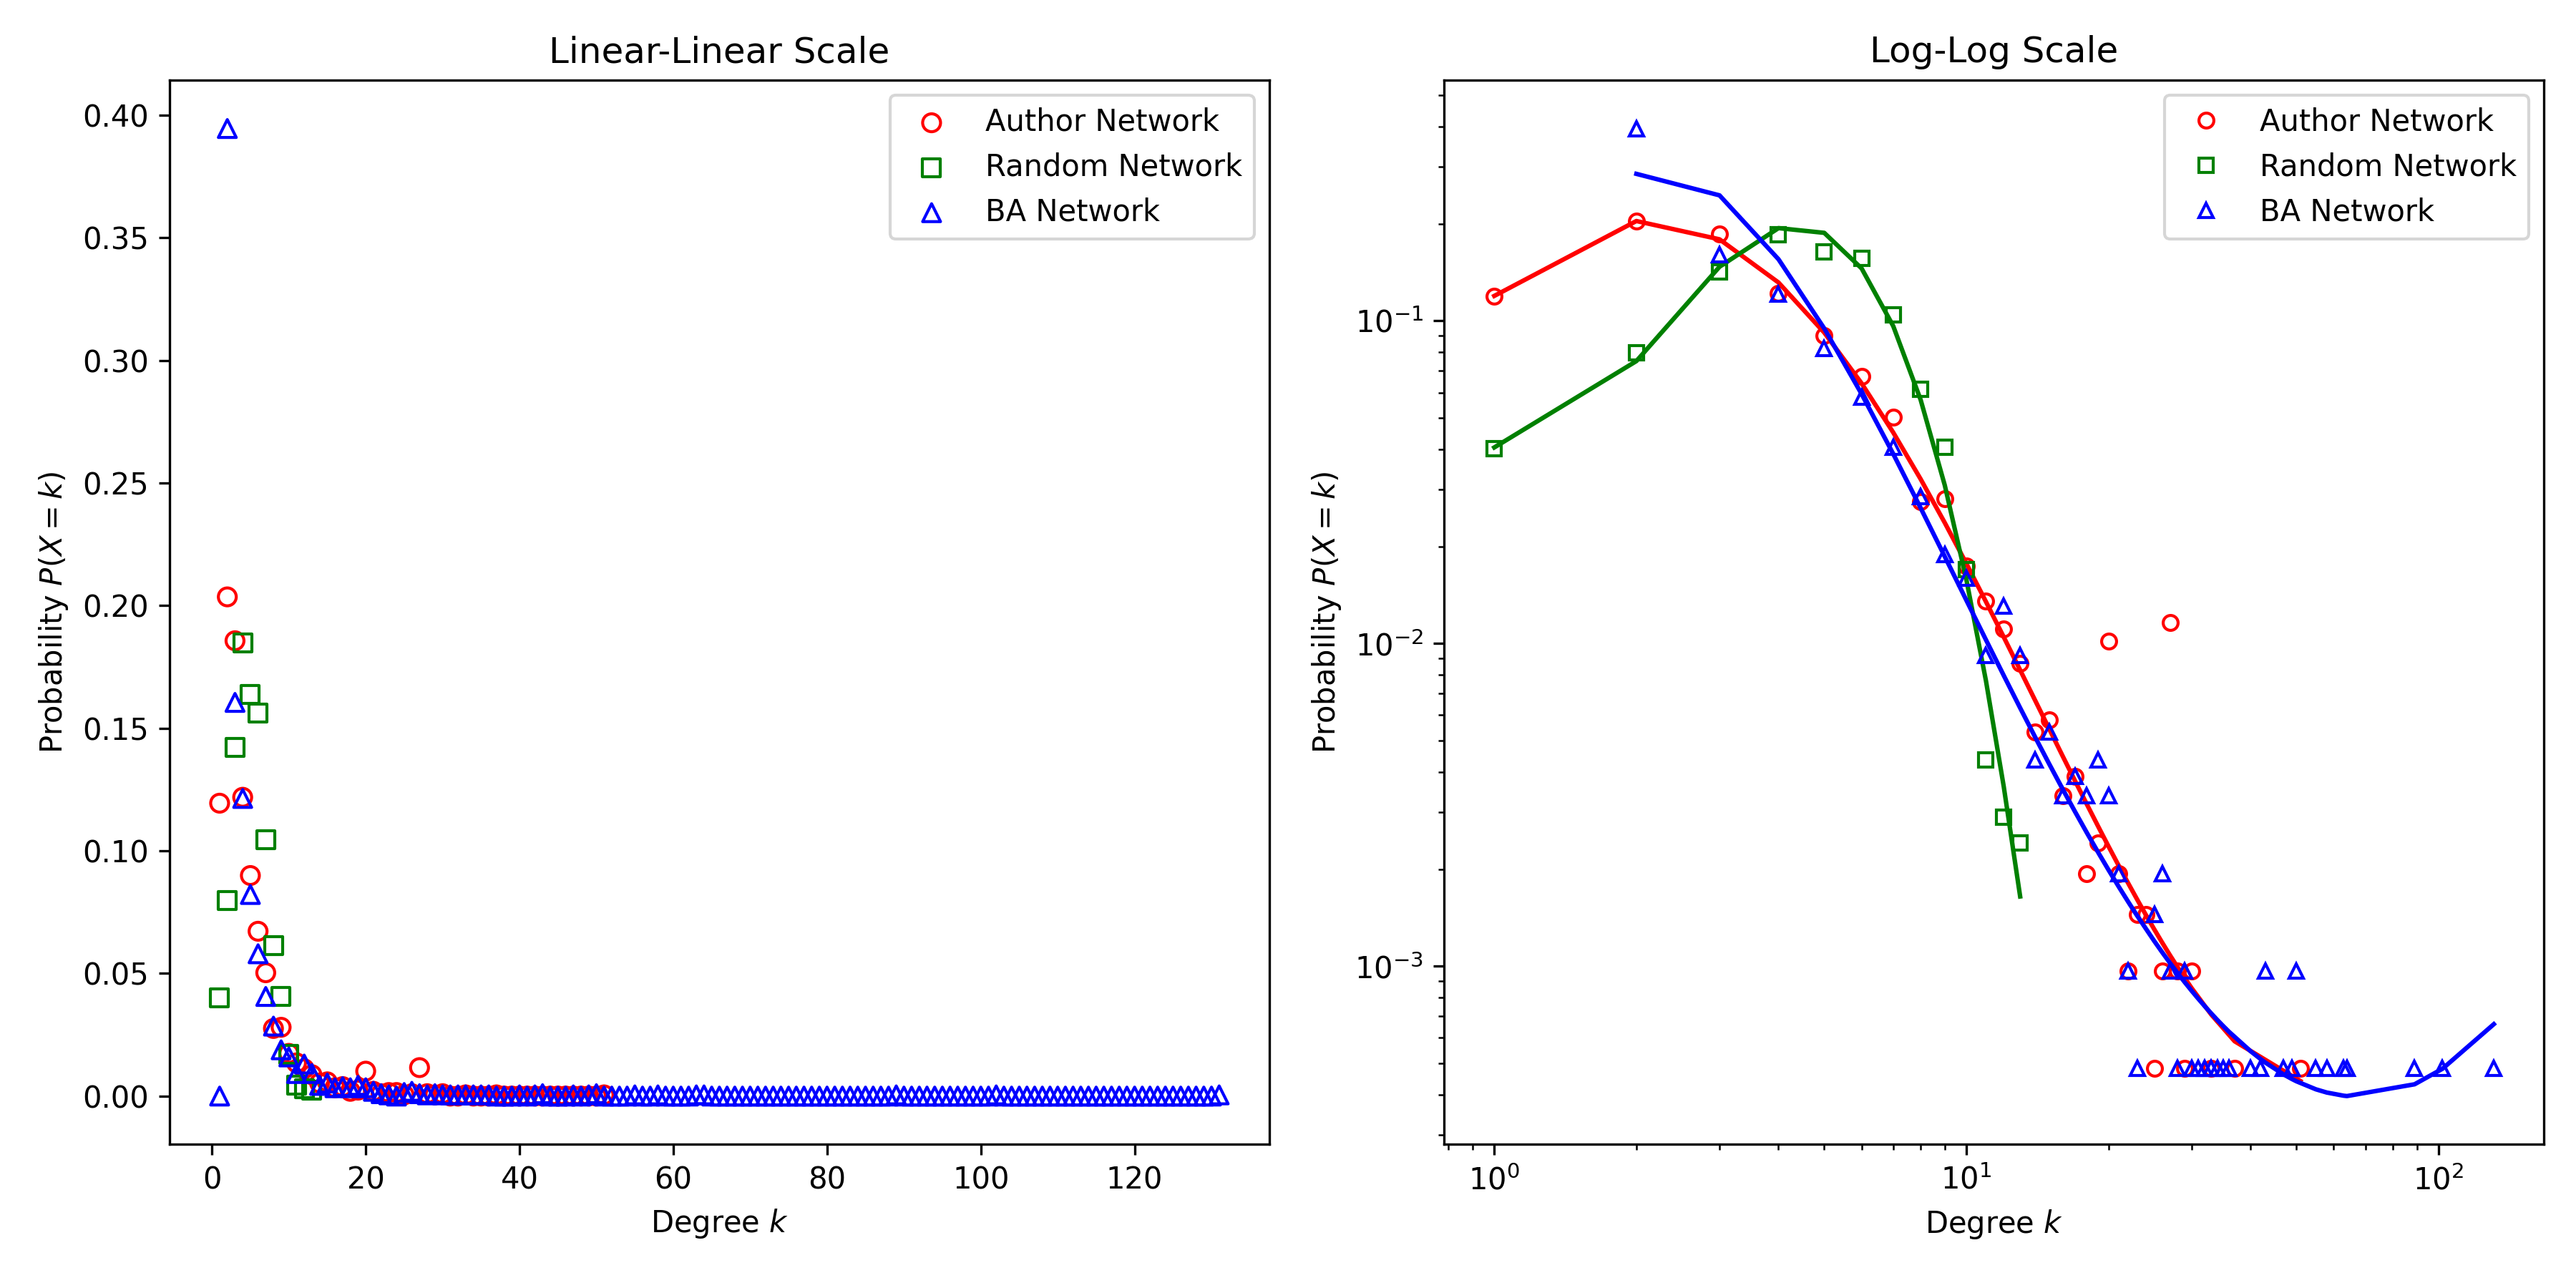
\includegraphics[width=1\textwidth]{degree_distributions.png}
    \label{fig:Degree_Distribution}
\end{figure}

\paragraph{}We estimate the power-law exponent to be $\alpha = 2.01$ for the author network.

\section*{Task 2 - (15 marks)}
\fbox{%
  \parbox{1\textwidth}{%
  \begin{itemize}
	\item Calculate and plot the nearest neighbour's average degree $k_{nn}$ as a function of degree $k$, on log-log scale.
	\item Calculate the assortative coefficient of the networks.
	\item Briefly discuss your results
\end{itemize}
  }%
}

\begin{figure}[h]
    \centering
    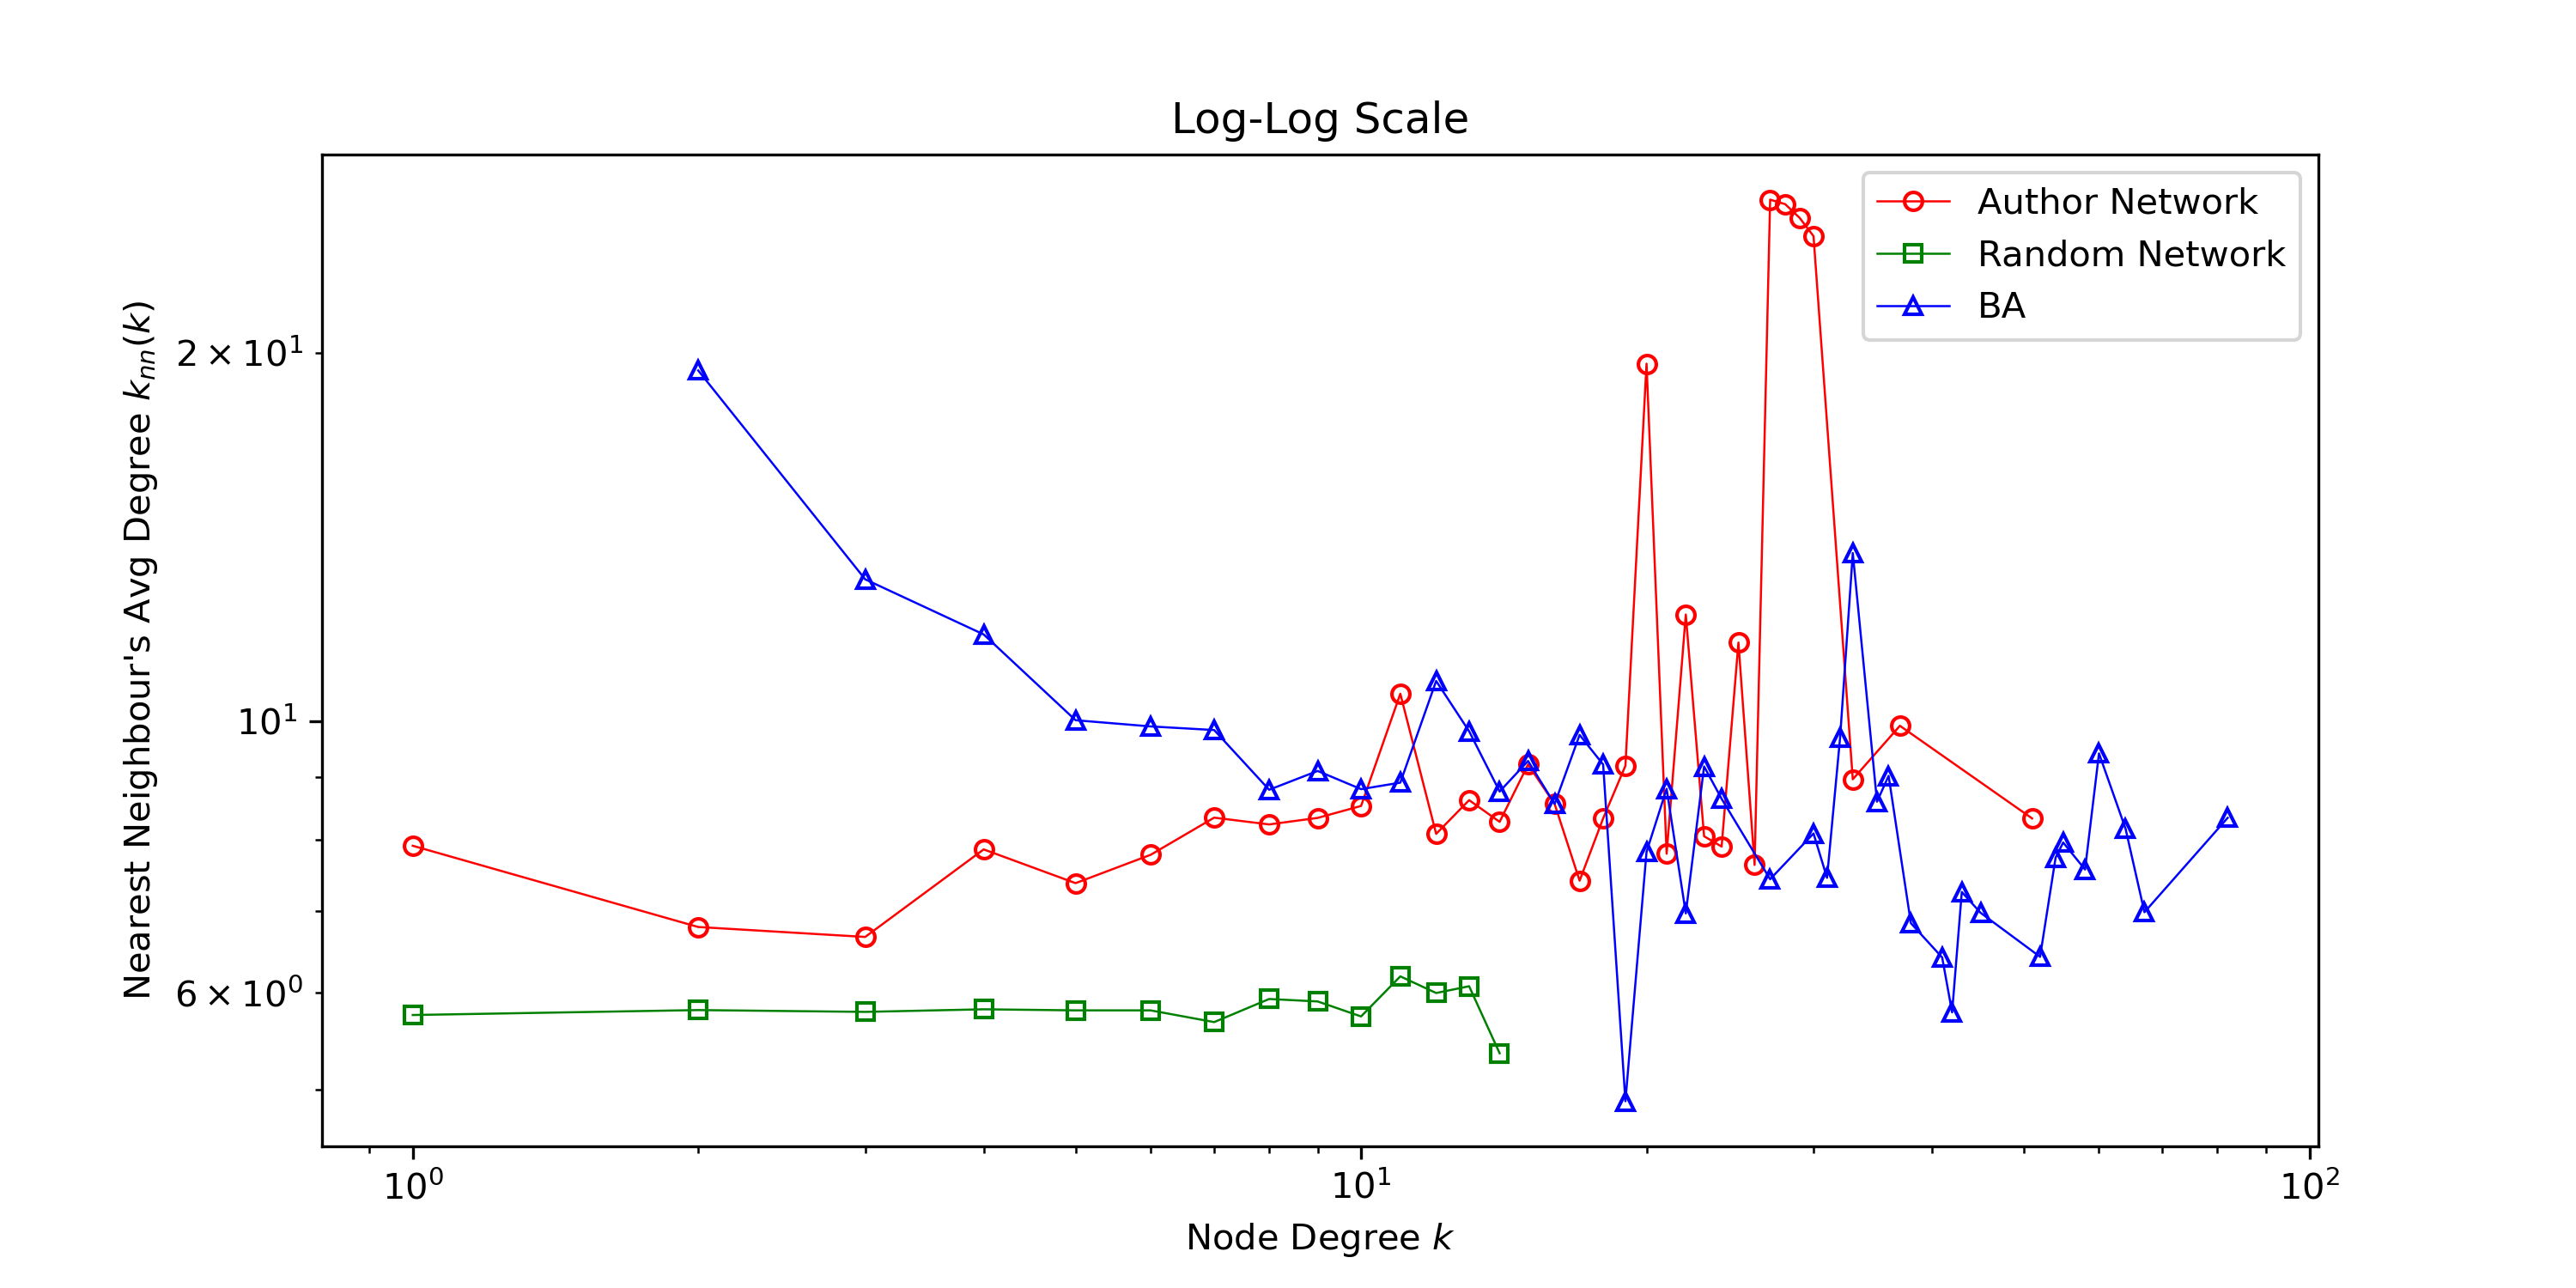
\includegraphics[width=1\textwidth]{nearest_neighbours_average_degree.png}
    \label{fig:Nearest Neighbours Average Degree}
\end{figure}

\begin{center}
\begin{tabular}{ | m{15em} | m{15em} | } 
  \hline
  \textbf{Networks} & \textbf{Assortative Coefficient} \\
  \hline 
  Author Network & \ \ 0.47 \\ 
  \hline
  Random Network & \ \ 0.01 \\ 
  \hline
  BA Network & - 0.16 \\
  \hline
\end{tabular}
\end{center}


\section*{Task 3 - (15 marks)}
\fbox{%
  \parbox{1\textwidth}{%
  	\begin{itemize}
	\item Calculate the diameter and the average shortest path length of the network
	\item Calculate and plot the average node between of $k$-degree nodes as a function of node degree $k$, where node betweenness is normalised, on log-log scale.
	\item Briefly discuss your results.
	\end{itemize}
  }%
}

\begin{center}
	\begin{tabular}{ | m{11em} | m{11em} | m{13em} | } 
  	\hline
  	\textbf{Networks} & \textbf{Diameter} & \textbf{Avg Shortest Path Length}\\
  	\hline 
  	Author Network & 19 & 7.30 \\ 
  	\hline
  	Random Network & 10 & 4.93 \\ 
  	\hline
  	BA Network & 10 & 4.56 \\
  	\hline
	\end{tabular}
\end{center}

\begin{figure}[h]
    \centering
    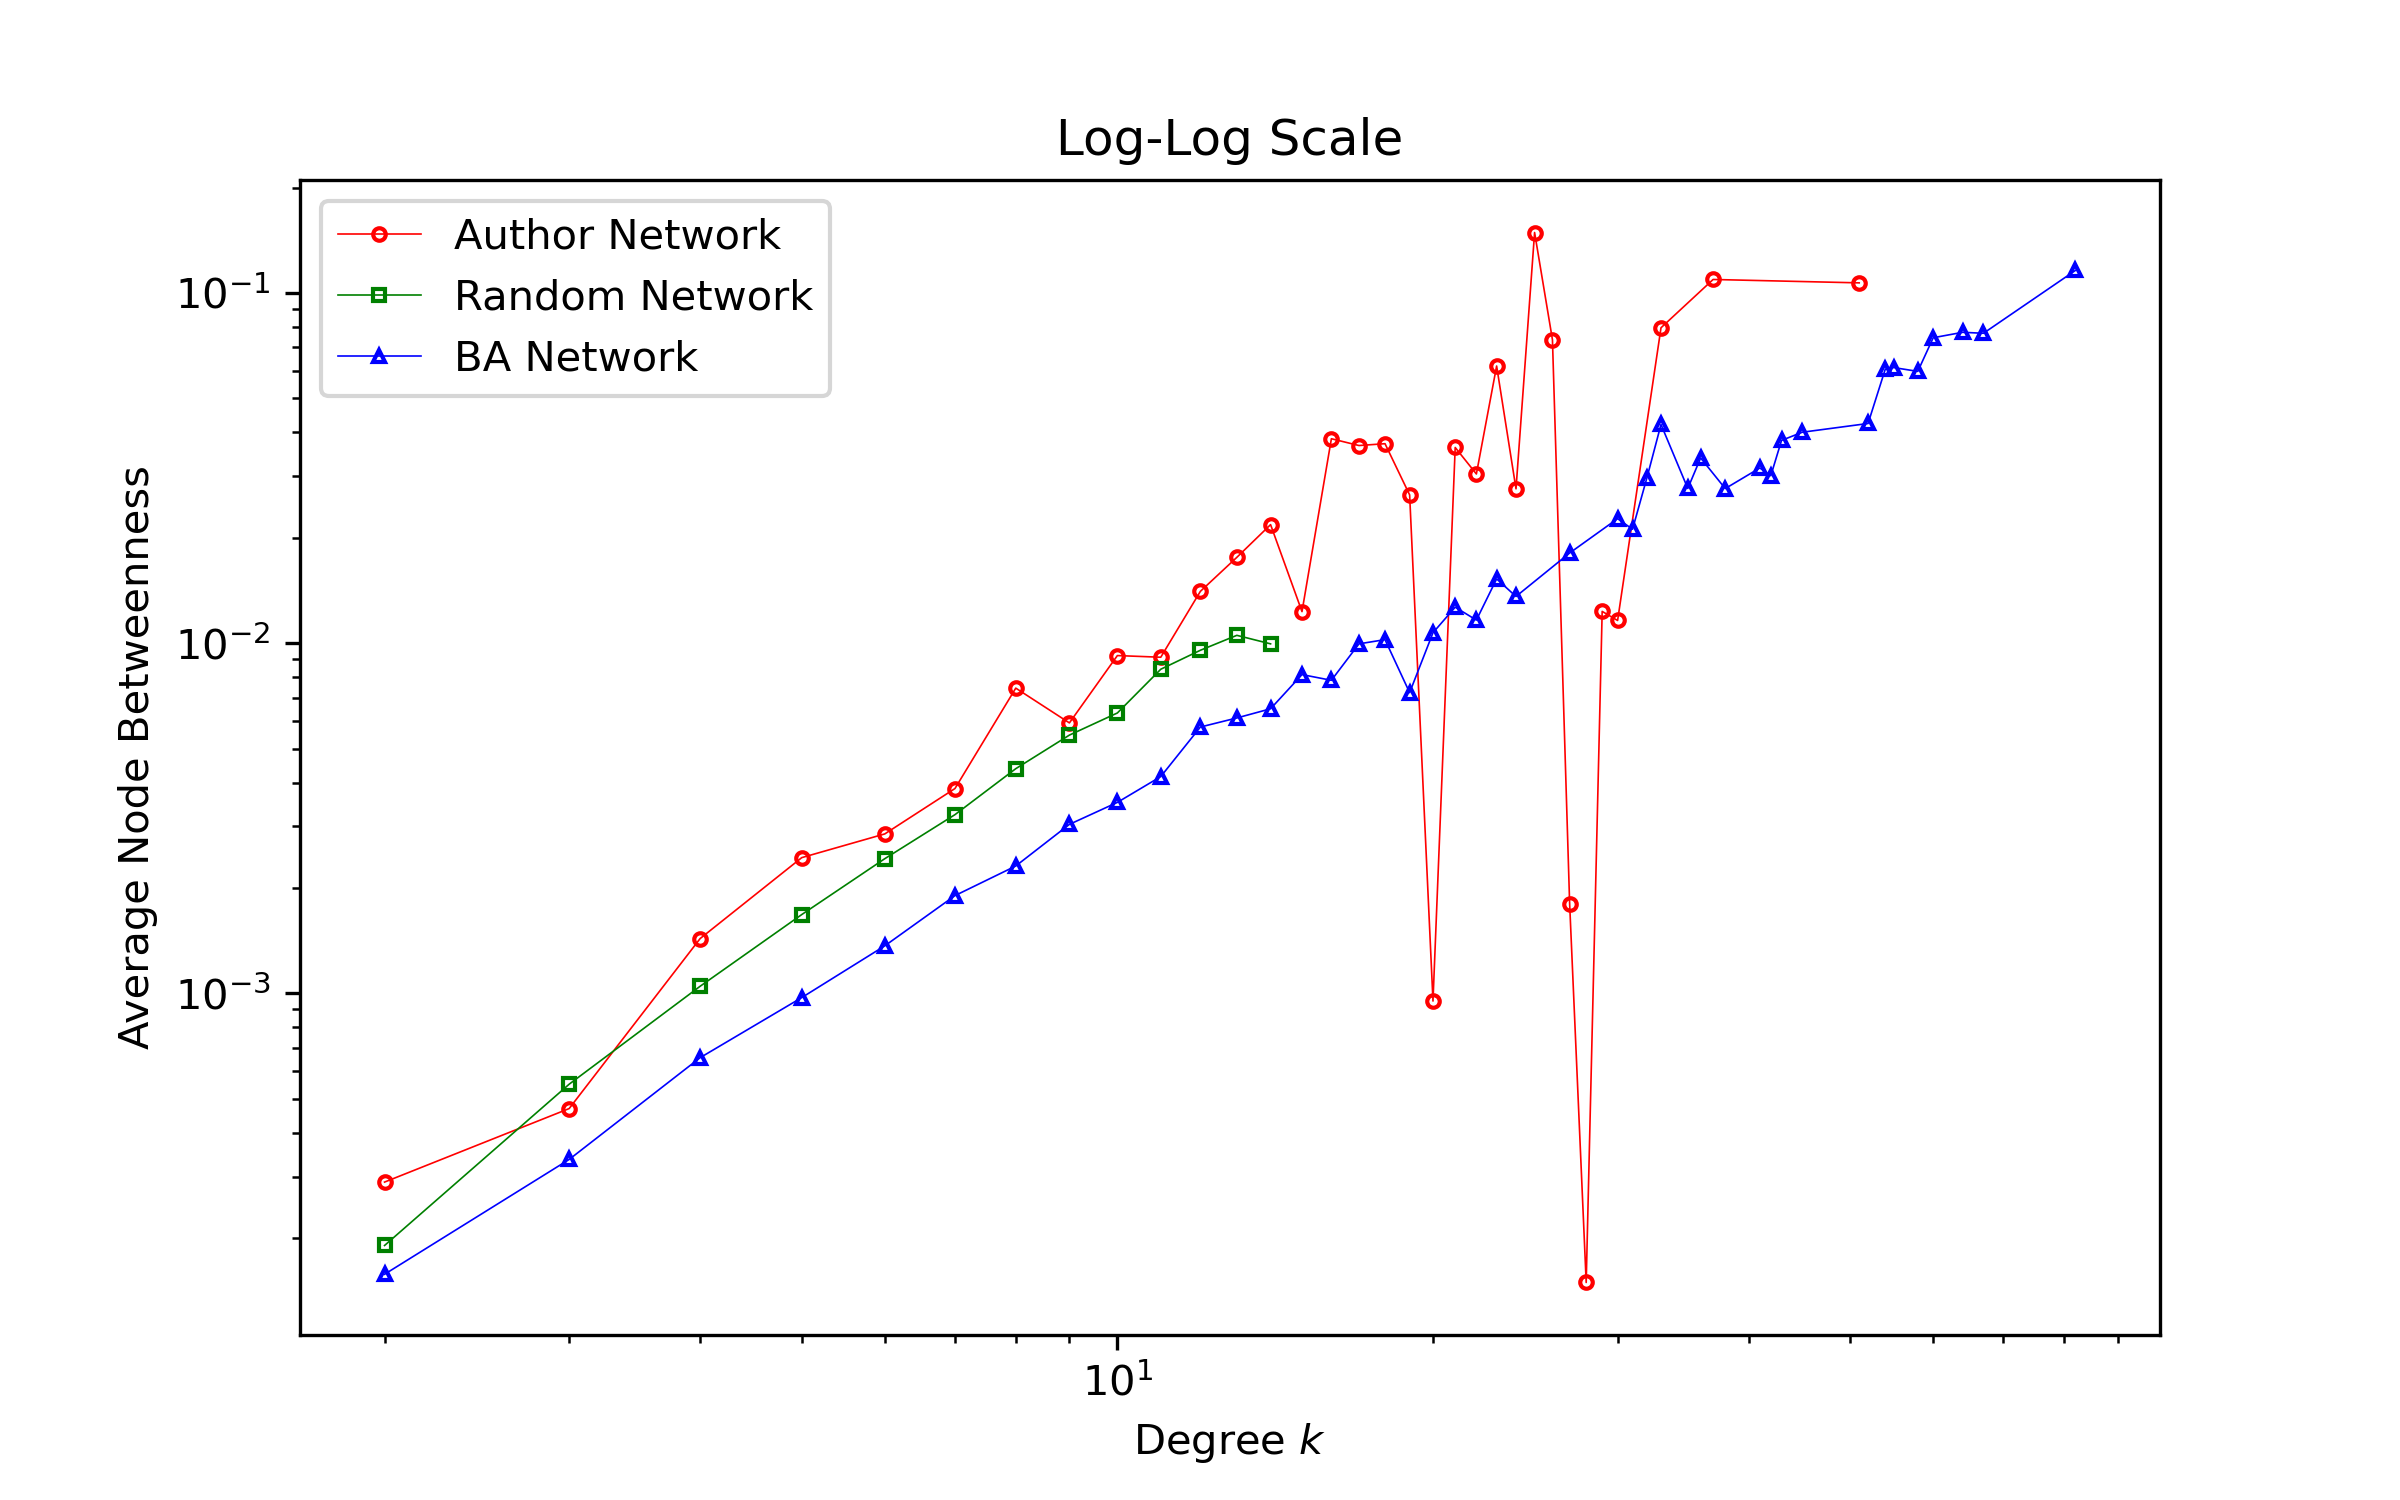
\includegraphics[width=1\textwidth]{average_node_betweenness.png}
    \label{fig:Averade Node Betweenness}
\end{figure}


\section*{Task 4 - (15 marks)}
\fbox{%
  \parbox{1\textwidth}{%
  \begin{itemize}
	\item Calculate and plot the rich-club coefficient as a function of node rank on log-log scale
	\item Calculate and plot the rich-club coefficient as a function of node degree on log-log scale
	\item Briefly discuss your result
\end{itemize}
  }%
}

\begin{figure}[h]
    \centering
    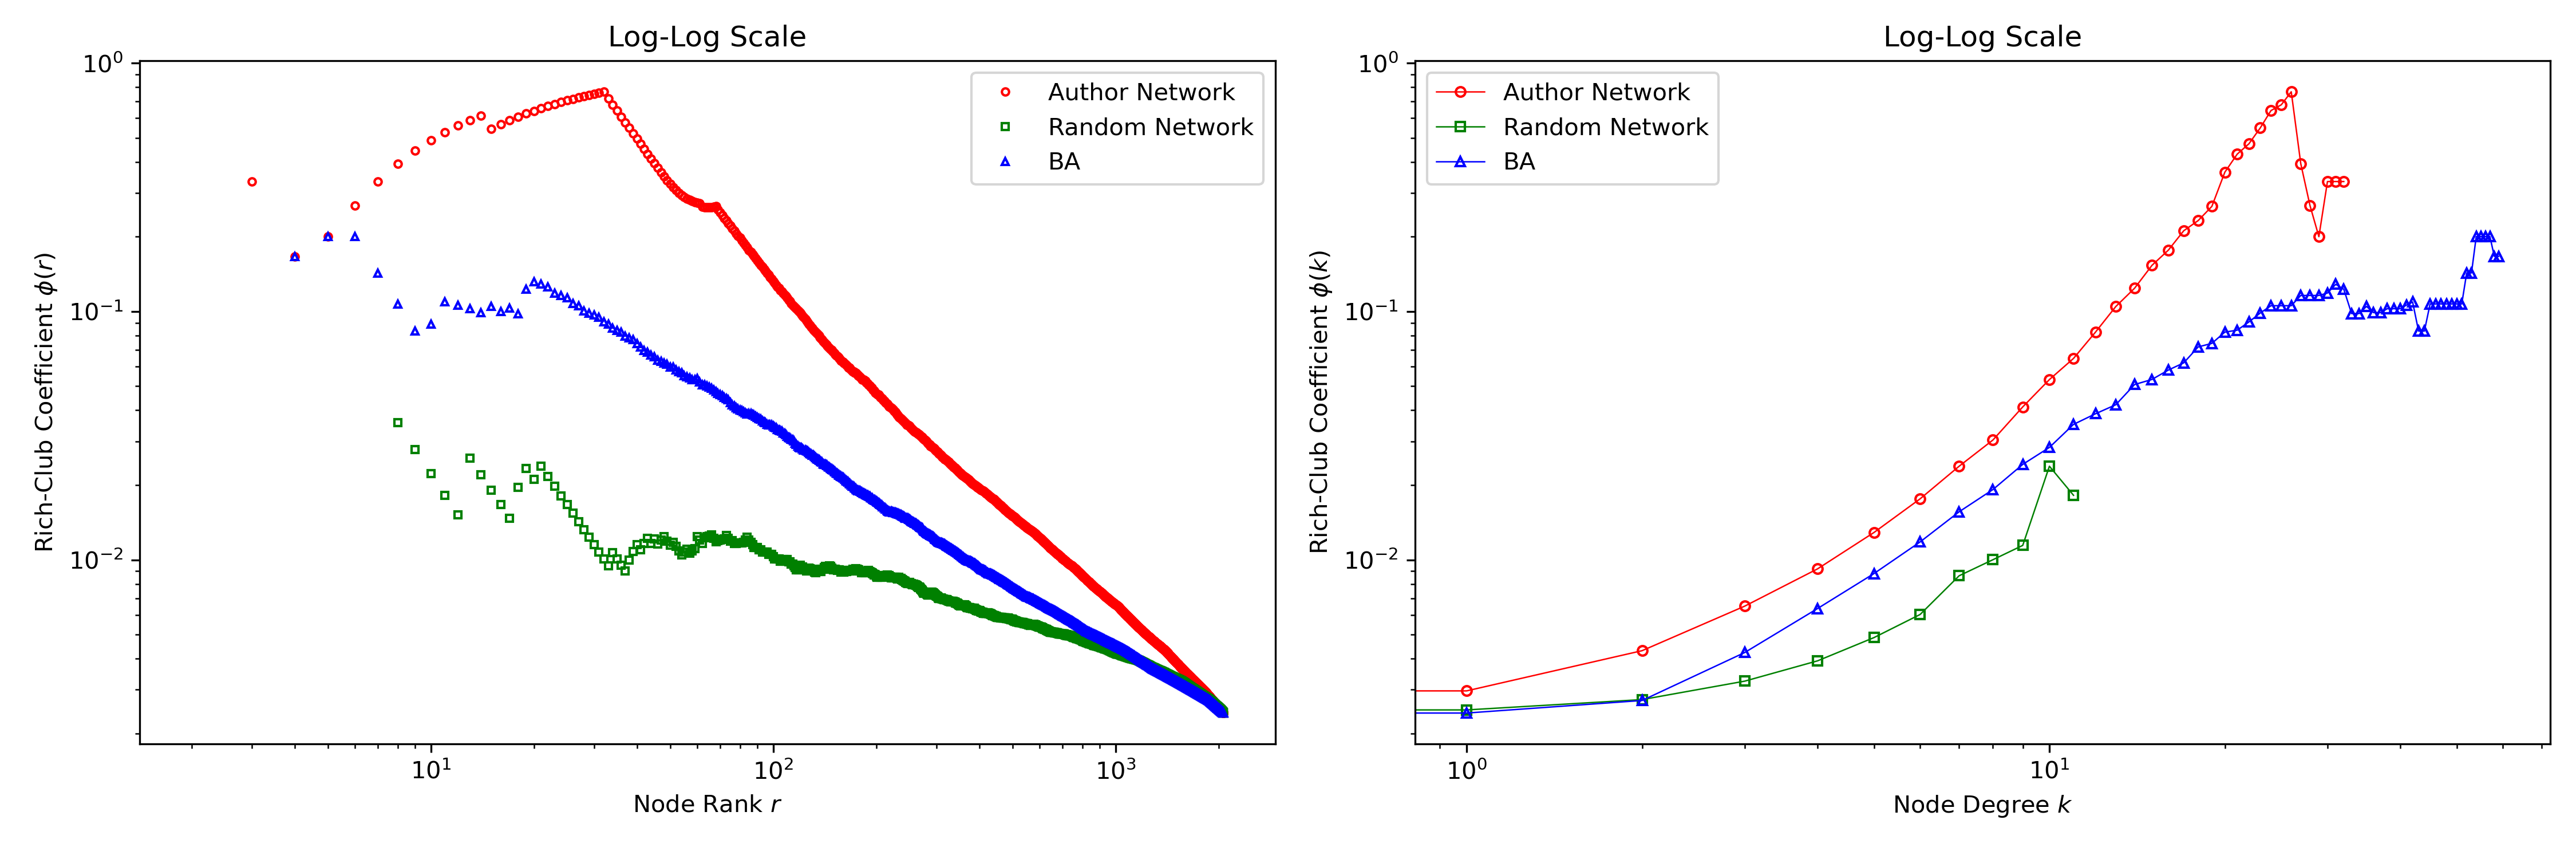
\includegraphics[width=1\textwidth]{rich_club.png}
    \label{fig:Rich-Club Coefficient}
\end{figure}

\section*{Task 5 - (15 marks)}
\fbox{%
  \parbox{1\textwidth}{%
  	\begin{itemize}
	\item Obtain the community structure (with the largest modularity value) of the 3 networks
	\item Give the number of communities and the size (i.e. number of nodes) of the top 3 largest communities in each netwoork.
	\item Visualise the network and show each community with a different colour.
	\item Briefly discuss your result
\end{itemize}
  }%
}

\section*{Task 6 - (25 marks)}

\fbox{%
	\parbox{1\textwidth}{%
	\begin{itemize}
	\item Randomly rewire the 3 networks while preserving the degree distribution; and obtain the maximal random case of each network
	\item For the 3 randomised networks, plot their degree distribution
	\item Calculate the average clustering coefficient, the assortative coefficient, and the average shortest path length of the 3 networks and the 3 randomised networks; show and compare the results in a table
	\item Briefly discuss you result.
\end{itemize}
	}%
}

\begin{figure}[h]
    \centering
    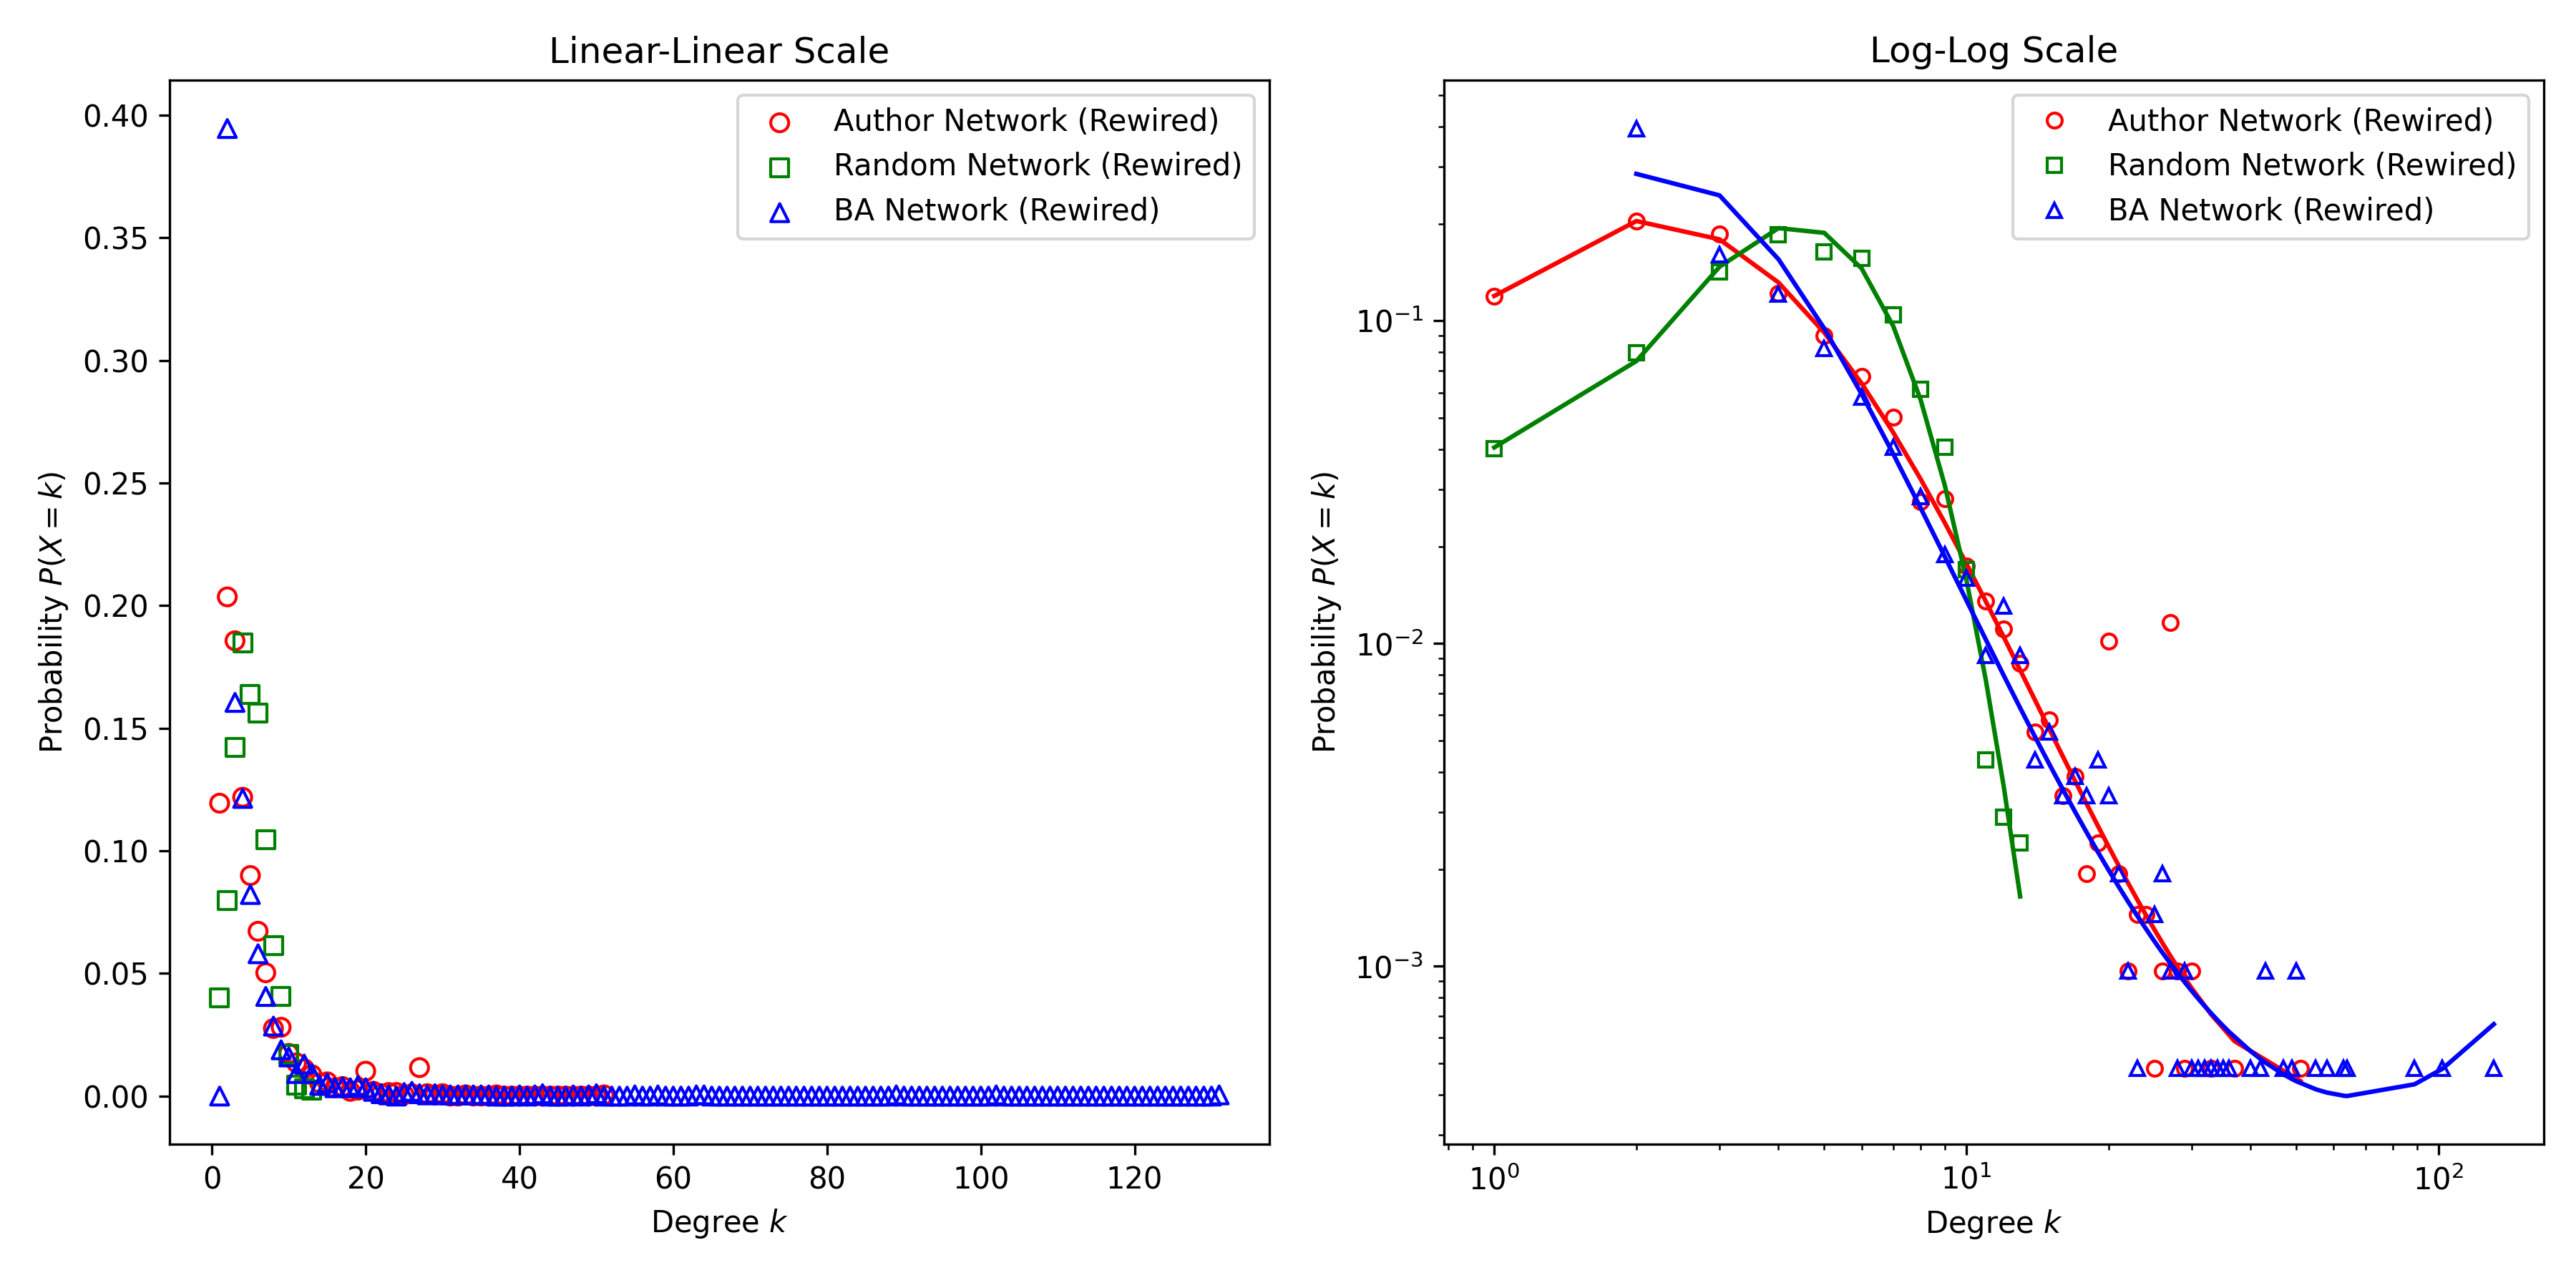
\includegraphics[width=1\textwidth]{degree_distributions_rewired}
    \label{fig:Degree Distributions (Rewired Networks)}
\end{figure}

\begin{center}
	\begin{tabular}{ | m{12em} | m{8em} | m{7em} | m{10em} | } 
  	\hline
  	\textbf{} & \textbf{Avg Clustering Coefficient} & \textbf{Assortative Coefficient} & \textbf{Avg Shortest Path Length} \\
  	\hline 
  	Author Network & 0.62 & \ 0.47 & 7.30 \\ 
  	\hline
  	Author Network (rewired) & 0.01 & \ 0.05 & 4.43 \\ 
  	\hline
  	Random Network & 0.00 & \ 0.01 & 4.93 \\
  	\hline
  	Random Network (rewired) & 0.00 & -0.03 & 4.94 \\
  	\hline
  	BA Network & 0.01 & -0.16 & 4.56 \\
  	\hline
  	BA Network (rewired) & 0.00 & -0.13 & 4.55 \\
  	\hline
	\end{tabular}
\end{center}

\paragraph{}


\bibliographystyle{acm}
\bibliography{references}

\end{document}